\chapter{Introduction}
% This magic comment tells some compilers to build the main document on save instead
% of trying to build the current tex file, which will fail because it isn't stand-alone
% !TEX root = master.tex

\section{Outline}

This chapter describes the basics of using the template to meet BYU's
thesis formatting requirements. There is also a good deal of filler text to
make it look like a full document. The first paragraphs of each section discuss
real stuff.

\subsection{Title Styles}

All the titles in this document use a defined style.  Use the \verb+\chapter{}+
command for chapters, \verb+\section{}+ for sections, and \verb+\subsection{}+
for second-level headings.

\subsubsection{Outline styles}

The \texttt{byuthesis} class does define a third-level heading
at \verb+\subsubsection{}+, but there are no formatting instructions on this so
you probably want to skip it.

\subsection{Filler}

\lipsum[3]

\section{Floating environments}

\LaTeX allows users to create tables and insert figures into their documents.
Floats should be at the top of the page or on their own pages, which \LaTeX will
do automatically. Use the \LaTeX \ figure referencing / labels system to make your life easy. Labelled figures and tables will also be automatically
added to the relevant list in the thesis frontmatter.

\subsection{Figures}

Figures
can be included with the standard \LaTeX \ figure commands; every figure should
be referred to in the text, such as the diagram of sudden infant death
syndrome (SIDS) incidence rates in North Carolina show in Figure \ref{fig:ncplot}.
Figure captions should be one or more
sentences that end in a period.

\begin{figure}
  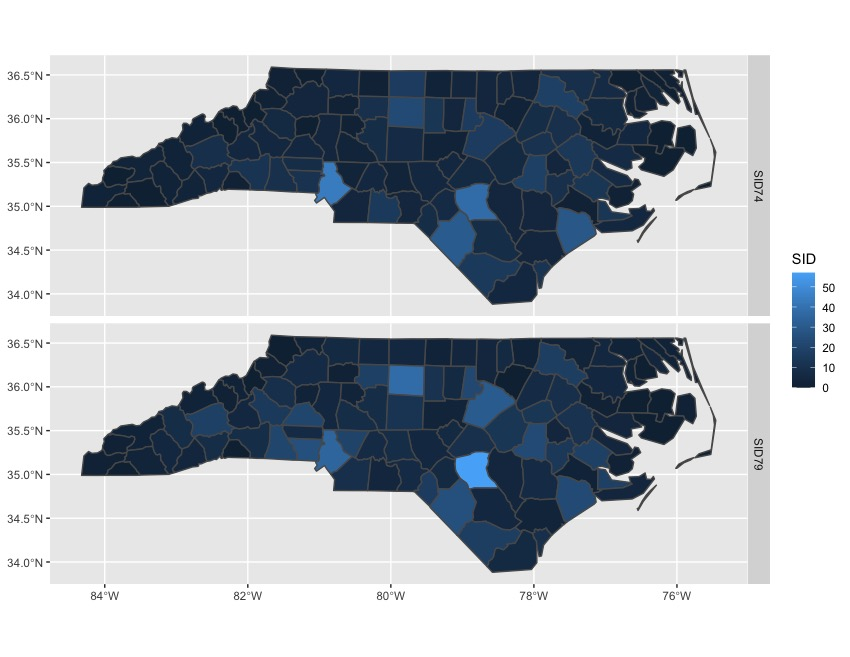
\includegraphics[width=\textwidth]{./images/ncplot}
  \caption{\label{fig:ncplot} Incidence of SIDS in North Carolina.}
\end{figure}


\subsection{Tables}

Tables can also be included with the standard \LaTeX \ table commands, with
references and labels. The thesis class equips the recommended
\texttt{booktabs} library, which includes commands to introduce horizontal
rules in tables. Table captions should be like titles. Tables should also
be referenced in the text, using the standard reference command to refer
to Table \ref{tab:example}.

\begin{table}
  \begin{center}
\caption{\label{tab:example} An Example Table}
\begin{tabular}{lcccccl}
  \toprule
& \multicolumn{3}{c}{$tol=tols$} & \multicolumn{3}{c}{$tol=told$}
\\\cmidrule(lr){2-4}
\cmidrule(lr){5-7}
           & $mv$  & Rel.~err & Time    & $mv$  & Rel.~err & Time\\
\midrule
trigmv    & 11034 & 1.3e-7 & 3.9 & 15846 & 2.7e-11 & 5.6 \\
trigexpmv & 21952 & 1.3e-7 & 6.2 & 31516 & 2.7e-11 & 8.8 \\
trigblock & 15883 & 5.2e-8 & 7.1 & 32023 & 1.1e-11 & 1.4e1\\
expleja   & 11180 & 8.0e-9 & 4.3 & 17348 & 1.5e-11 & 6.6 \\
\bottomrule
\end{tabular}
\end{center}
\end{table}

\section{Extra filler}
\lipsum
